% =====================================================================
%  Optimal Crop-Area Allocation for Agricultural Resource Planning
%  IEEE conference format (IEEEtran).  Compile with pdfLaTeX (Overleaf:
%  upload this folder, set main.tex as the main document).
%  Figures in ./figures are produced by make_figures.py (vector PDF).
% =====================================================================
\documentclass[conference]{IEEEtran}
\IEEEoverridecommandlockouts

\usepackage{cite}
\usepackage{amsmath,amssymb,amsfonts}
\usepackage{graphicx}
\usepackage{booktabs}
\usepackage{multirow}
\usepackage{array}
\usepackage{xcolor}
\usepackage{url}
\usepackage{tikz}
\usetikzlibrary{arrows.meta,positioning,shapes.geometric,fit}
\usepackage[hidelinks]{hyperref}

\graphicspath{{figures/}}
% line break between author rows (standard IEEEtran workaround)
\makeatletter
\newcommand{\linebreakand}{%
  \end{@IEEEauthorhalign}\hfill\mbox{}\par\mbox{}\hfill\begin{@IEEEauthorhalign}}
\makeatother
\definecolor{orblue}{HTML}{2A78D6}
\definecolor{ororange}{HTML}{EB6834}
\newcommand{\Lhist}{L_{\mathrm{hist}}}
\newcommand{\Dhist}{D_{\mathrm{hist}}}

\begin{document}

\title{Optimal Crop-Area Allocation for Agricultural Resource Planning:\\
A Linear Programming Approach using District-Level Crop Production Data of the Government of India}

\author{
\IEEEauthorblockN{Nitin Krishna V}
\IEEEauthorblockA{CB.SC.U4AIE23156}
\and
\IEEEauthorblockN{Vishal Suresh}
\IEEEauthorblockA{CB.SC.U4AIE23160}
\and
\IEEEauthorblockN{Manogna Challa}
\IEEEauthorblockA{CB.SC.U4AIE23175}
\and
\IEEEauthorblockN{Gaurav Mahesh}
\IEEEauthorblockA{CB.SC.U4AIE23176}
\linebreakand
\IEEEauthorblockA{\textit{Department of Computer Science and Engineering (Artificial Intelligence)}\\
\textit{Amrita School of AI, Amrita Vishwa Vidyapeetham}\\
Coimbatore, India}
}

\maketitle

% ---------------------------------------------------------------------
\begin{abstract}
Cultivable land is fixed while crop yields differ sharply across crops, districts and
years, yet seasonal land allocation is usually decided by habit rather than by evidence.
This paper builds two linear programming (LP) models---maximisation of total output for a
fixed land budget, and minimisation of land for a production target---whose coefficients
are taken entirely from the Government of India's district-wise, season-wise crop
production record (575{,}879 rows, 1997--2020). Before modelling, a systematic data audit
revealed that the public file consists of two stacked copies of the same records, one with
production inflated by a factor of 100; an automatic reconciliation procedure is proposed
that restores a single consistent unit. Crops reported in count or bale units are excluded
by a two-test production-unit check. For Karnataka's Kharif season (1998--2019, 19 crops),
the output-maximising plan raises production by 21.6\% on the same land, and the
land-minimising plan meets historical output on 23.9\% less land. The two models are shown
to be linked exactly by duality ($\mu^*=1/\lambda^*$). Parametric analysis, coefficient
ranging, yield-shock scenarios and a 27-district comparison show that the gain falls to
about 6\% when each crop may move only $\pm10\%$ from its historical area, in line with
published LP crop-planning studies. All models are delivered in an interactive,
upload-driven decision-support dashboard.
\end{abstract}

\begin{IEEEkeywords}
linear programming, crop planning, land allocation, sensitivity analysis, duality,
agricultural data quality, decision support system
\end{IEEEkeywords}

% =====================================================================
\section{Introduction}
% =====================================================================
Land is the binding resource of agriculture: a hectare given to one crop is a hectare
taken from another. Yield per hectare varies widely across crops, districts and years, and
India publishes these yields at district--season--year granularity. Nevertheless, the
allocation of land for the next season is rarely re-planned from such records.

This work asks: \emph{using actual historical yield records, how should land be
re-allocated across crops to obtain the most from a fixed area?} We answer it with linear
programming (LP)~\cite{taha2017}, in two complementary directions:
\begin{itemize}
  \item \textbf{Optimization~1:} maximise total production for a given land budget $L$;
  \item \textbf{Optimization~2:} minimise the land needed to guarantee a production target $D$.
\end{itemize}

The contributions of this paper are:
\begin{enumerate}
  \item a reproducible LP formulation built \emph{only} from area, production and yield in a
        public government dataset, with cost and profit deliberately left out because the data
        do not contain them;
  \item the discovery and automatic repair of a stacked-duplicate-source defect affecting
        212{,}373 records of the public dataset, together with a two-test production-unit check;
  \item a case study with primal--dual verification, sensitivity analysis and a multi-district
        comparison;
  \item an interactive dashboard in which any uploaded dataset is cleaned, explored and optimised.
\end{enumerate}

The rest of the paper is organised as follows. Section~\ref{sec:related} reviews related work.
Section~\ref{sec:data} describes the dataset and its quirks. Section~\ref{sec:model} gives the
formulation, and Section~\ref{sec:method} the solution method. Sections~\ref{sec:results}--\ref{sec:multi}
report results, Section~\ref{sec:tool} presents the dashboard, Section~\ref{sec:valid} validates the
pipeline on synthetic data, and Sections~\ref{sec:disc}--\ref{sec:concl} discuss limitations and conclude.

% =====================================================================
\section{Related Work}\label{sec:related}
% =====================================================================
LP has a long history in farm and regional crop planning. Wankhade and
Lunge~\cite{wankhade2012} allocated resources among ten crops in Akola district,
Maharashtra, showing that LP works on Indian district-level data. Majeke
\textit{et~al.}~\cite{majeke2020} found that an LP land-allocation plan outperformed a
small-holder's own plan. Supriya \textit{et~al.}~\cite{supriya2022} reported returns
improved by 3.75--15\% from LP crop plans in Telangana. Paidipati and
Padi~\cite{paidipati2017} formulated two LP models---cost minimisation and revenue
maximisation---motivating a primal/dual pair of objectives. Liang~\cite{liang2023} applied
LP to production--land allocation.

\textbf{Research gap.} These studies use a one-time survey of a single district and assume
known prices. None derives its coefficients from a multi-year, multi-district government
record, and none reports a systematic audit of the data before modelling. Our work builds
the LP strictly from a public record, keeps cost and profit out rather than approximating
them, and makes the analysis reproducible and interactive.

% =====================================================================
\section{Dataset and Data Preparation}\label{sec:data}
% =====================================================================
\subsection{Dataset}
The \emph{District-wise, Season-wise Crop Production Statistics} of the Ministry of
Agriculture \& Farmers Welfare~\cite{moafw} (via data.gov.in and Kaggle) is summarised
in Table~\ref{tab:dataset}. In every row, \texttt{yield}~$=$~\texttt{Production}/\texttt{Area}
exactly.

\begin{table}[t]
\centering
\caption{Dataset summary}\label{tab:dataset}
\begin{tabular}{@{}ll@{}}
\toprule
Rows $\times$ columns & 575{,}879 $\times$ 8, no missing values\\
Coverage & 36 states/UTs, 730 districts, 128 crop names\\
Years & crop years 1997--2020\\
Seasons & Kharif, Rabi, Whole Year, Summer, Winter, Autumn\\
Fields & State, District, Year, Season, Crop,\\
       & Area (ha), Production, Yield\\
\bottomrule
\end{tabular}
\end{table}

\subsection{Pipeline}
Fig.~\ref{fig:workflow} shows the workflow. Each step is implemented as a pure function in
\texttt{or\_core.py} and logged, so that every removed or modified row is traceable
(Table~\ref{tab:cleaning}).

\begin{figure}[t]
\centering
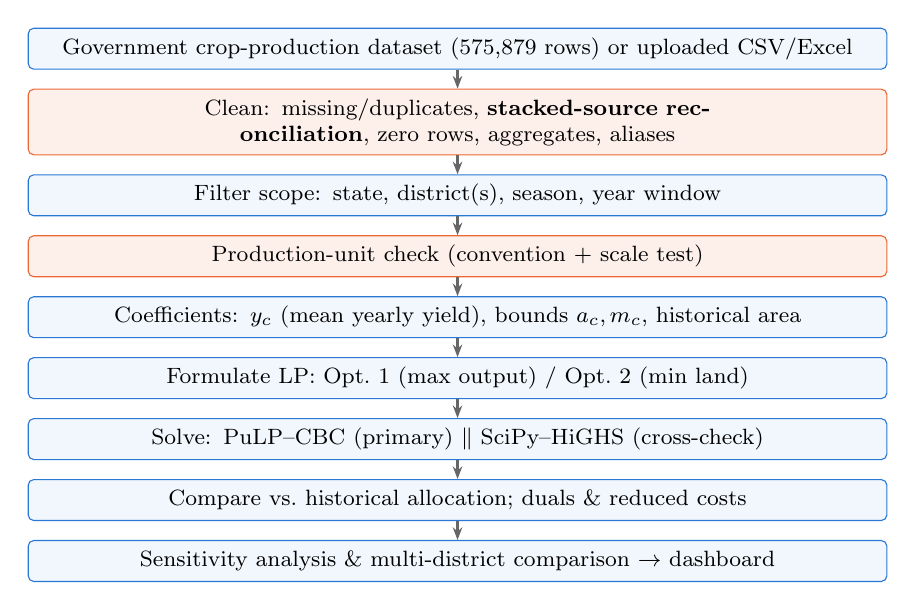
\begin{tikzpicture}[
  node distance=2.4mm,
  box/.style={draw=orblue, rounded corners=2pt, fill=orblue!6, text width=0.88\columnwidth,
              minimum height=5.2mm, align=center, font=\footnotesize},
  hl/.style={box, draw=ororange, fill=ororange!10},
  arr/.style={-{Stealth[length=1.6mm]}, thick, draw=black!60}]
\node[box] (a) {Government crop-production dataset (575{,}879 rows) or uploaded CSV/Excel};
\node[hl, below=of a] (b) {Clean: missing/duplicates, \textbf{stacked-source reconciliation}, zero rows, aggregates, aliases};
\node[box, below=of b] (c) {Filter scope: state, district(s), season, year window};
\node[hl, below=of c] (d) {Production-unit check (convention + scale test)};
\node[box, below=of d] (e) {Coefficients: $y_c$ (mean yearly yield), bounds $a_c, m_c$, historical area};
\node[box, below=of e] (f) {Formulate LP: Opt.~1 (max output) / Opt.~2 (min land)};
\node[box, below=of f] (g) {Solve: PuLP--CBC (primary) $\Vert$ SciPy--HiGHS (cross-check)};
\node[box, below=of g] (h) {Compare vs.\ historical allocation; duals \& reduced costs};
\node[box, below=of h] (i) {Sensitivity analysis \& multi-district comparison $\rightarrow$ dashboard};
\foreach \u/\v in {a/b,b/c,c/d,d/e,e/f,f/g,g/h,h/i} \draw[arr] (\u) -- (\v);
\end{tikzpicture}
\caption{Project workflow. Highlighted steps are the data-quality safeguards applied
before any coefficient is built.}
\label{fig:workflow}
\end{figure}

\begin{table}[t]
\centering
\caption{Cleaning log on the GOV dataset}\label{tab:cleaning}
\begin{tabular}{@{}lr@{}}
\toprule
Step & Rows removed\\
\midrule
Missing crop / area / production & 0\\
Exact duplicate rows & 0\\
\textbf{Stacked duplicate source (Sec.~\ref{sec:stacked})} & \textbf{212{,}373}\\
Area $\le 0$ & 0\\
Production $=0$ (mostly unreported) & 3{,}634\\
Aggregate rows (Total foodgrain, Pulses/Oilseeds total) & 1{,}133\\
Spelling variants merged (e.g.\ Paddy$\to$Rice) & 3{,}565 renamed\\
\midrule
Rows after cleaning & 358{,}739\\
\bottomrule
\end{tabular}
\end{table}

\subsection{Stacked Duplicate Source}\label{sec:stacked}
Plotting pooled yield over time showed an apparent doubling in 2015
(Fig.~\ref{fig:stacked}b). Closer inspection showed that the file is the concatenation of
two blocks:
\begin{itemize}
  \item rows 0--236{,}377 (1997--2015);
  \item rows 236{,}378--575{,}878 (1997--2020).
\end{itemize}
212{,}373 records occur in both blocks with identical state, district, year, season, crop
\emph{and} area, and in 99.4\% of these pairs the second copy's production is exactly
$100\times$ the first. Because the second block is the only source after 2014, the raw data
show a spurious ``break'', and years before 2015 carry twice the records
(Fig.~\ref{fig:stacked}a).

The proposed reconciliation proceeds in five steps:
\begin{enumerate}
  \item pair the records that share all six key fields;
  \item take the modal production ratio, snapped to a power of ten ($k=100$);
  \item check that the pairs split cleanly by row position;
  \item divide production in the second block by $k$;
  \item keep one record per pair.
\end{enumerate}
The reconciled series is smooth over 1998--2019 (Fig.~\ref{fig:stacked}c). National yields
then match published values in t/ha (rice 2.0--2.8, wheat 2.5--3.7, sugarcane
$\approx$70), which establishes that production is in tonnes. The remaining anomalies in
1997 and 2020 are partial-coverage years (2020 has only 319 rows), so the analysis window
is 1998--2019.

\begin{figure*}[t]
\centering
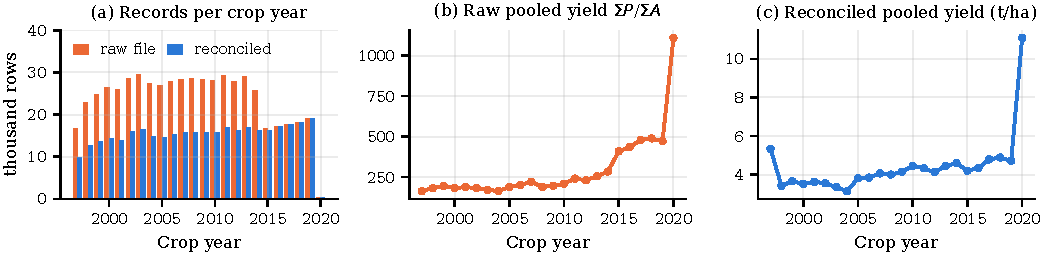
\includegraphics[width=\textwidth]{fig_stacked_source}
\caption{Stacked-duplicate-source defect in the public dataset.
(a) Records per crop year before and after reconciliation.
(b) Raw pooled yield $\sum P/\sum A$ over weight-unit crops, mixing two scales.
(c) Pooled yield after reconciliation, in t/ha.}
\label{fig:stacked}
\end{figure*}

\subsection{Production-Unit Consistency}
Only crops measured in the same production unit can be summed in one objective. Two tests
are applied:
\begin{enumerate}
  \item \emph{Convention test.} data.gov.in reports Coconut in nuts, Cotton (lint) and Kapas
        in bales of 170\,kg, and Jute, Mesta and Sannhamp in bales of 180\,kg.
  \item \emph{Scale test.} A crop is flagged if its median yield exceeds 250$\times$, or falls
        below 1/250, of the pool median.
\end{enumerate}
For the case study (Fig.~\ref{fig:unit}), Mesta and Cotton are excluded. Across the full
dataset, Coconut (median $\approx$6{,}500 nuts/ha versus $\approx$2.6\,t/ha for rice) is
excluded by both tests.

\begin{figure}[t]
\centering
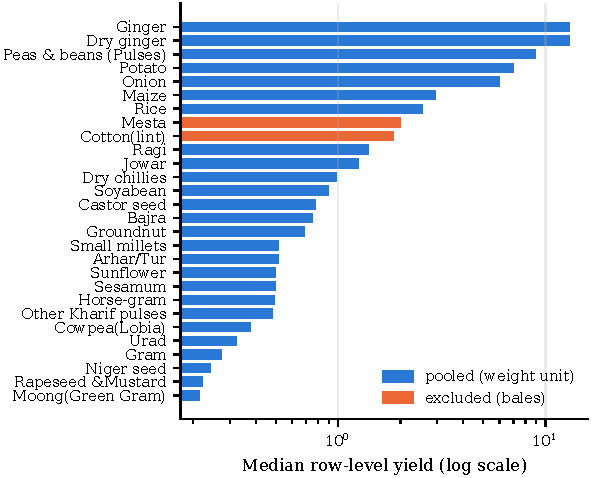
\includegraphics[width=\columnwidth]{fig_unit_check}
\caption{Production-unit check for Karnataka, Kharif, 1998--2019. Crops reported in bales
are excluded from the pooled LP.}
\label{fig:unit}
\end{figure}

\subsection{Coefficient Construction}
Records in the chosen scope are summed to crop--year level. For each crop $c$:
\begin{itemize}
  \item $y_c$ is the mean over years of $\sum P/\sum A$, i.e.\ the dataset's own yield averaged
        over the available years;
  \item $a_c$ and $m_c$ are the minimum and maximum yearly area;
  \item the historical allocation is the mean yearly area.
\end{itemize}
Crops observed in fewer than two thirds of the years are dropped, because their averages
are unstable.

% =====================================================================
\section{Mathematical Formulation}\label{sec:model}
% =====================================================================
Let $\mathcal{C}$ be the set of pooled crops in the chosen state and season, and let
$x_c\ge0$ be the hectares allotted to crop $c\in\mathcal{C}$.

\textbf{Optimization 1 (maximise output):}
\begin{align}
\max_{x}\quad & Z=\sum_{c\in\mathcal{C}} y_c\,x_c \label{eq:o1}\\
\text{s.t.}\quad & \sum_{c\in\mathcal{C}} x_c \le L \qquad (\lambda) \label{eq:land}\\
& a_c \le x_c \le m_c,\quad x_c\ge 0 \qquad \forall c\in\mathcal{C}. \label{eq:bounds}
\end{align}

\textbf{Optimization 2 (minimise land):}
\begin{align}
\min_{x}\quad & \sum_{c\in\mathcal{C}} x_c \label{eq:o2}\\
\text{s.t.}\quad & \sum_{c\in\mathcal{C}} y_c\,x_c \ge D \qquad (\mu) \label{eq:target}\\
& a_c \le x_c \le m_c,\quad x_c\ge 0 \qquad \forall c\in\mathcal{C}. \nonumber
\end{align}

By default, $L=\Lhist=\sum_c \bar{x}_c$ and $D=\Dhist=\sum_c y_c\bar{x}_c$, where $\bar{x}_c$
is the historical mean area.

\textbf{Solution structure.} With a single coupling constraint and box bounds,
\eqref{eq:o1}--\eqref{eq:bounds} is a continuous knapsack problem~\cite{dantzig1957}. The
optimum is obtained as follows:
\begin{enumerate}
  \item set every $x_c=a_c$;
  \item sort the crops by $y_c$;
  \item fill the remaining land from the highest-yield crop down, each up to $m_c$.
\end{enumerate}
The crop at which the land runs out is the unique basic variable, and its yield equals the
land dual $\lambda^*$. Crops with $y_c>\lambda^*$ end at $m_c$, and crops with
$y_c<\lambda^*$ end at $a_c$. The reduced cost of crop $c$ is $y_c-\lambda^*$.

Model \eqref{eq:o2}--\eqref{eq:target} has the same structure with land and output
exchanged. If Opt.~1 is solved with $L$ equal to the optimal land of Opt.~2, it returns
$Z^*=D$, and the duals satisfy
\begin{equation}
\mu^* = 1/\lambda^*. \label{eq:dual}
\end{equation}

% =====================================================================
\section{Solution Method and Tools}\label{sec:method}
% =====================================================================
Both LPs are solved with PuLP~\cite{pulp} using the CBC solver~\cite{cbc}, which provides
the duals and reduced costs. Every solve is repeated independently with SciPy's
\texttt{linprog}~\cite{scipy} using the HiGHS dual simplex~\cite{highs}. Across all runs,
the relative objective difference is below $10^{-9}$, and the two solvers' duals agree.

Parametric sweeps (60--120 solves each) use HiGHS in-process for speed. Data handling uses
pandas and NumPy, figures use Matplotlib and Plotly, and the interface is a FastAPI web
application with a hand-built HTML/JavaScript frontend.

% =====================================================================
\section{Results: Karnataka, Kharif, 1998--2019}\label{sec:results}
% =====================================================================
Nineteen pooled crops have at least 15 years of data. Their coefficients are listed in
Table~\ref{tab:coef} and plotted in Fig.~\ref{fig:coef}. The historical baseline is
$\Lhist=6{,}125{,}458$\,ha and $\Dhist=9{,}729{,}947$\,t.

\begin{table}[t]
\centering
\caption{LP coefficients (Karnataka, Kharif, 1998--2019)}\label{tab:coef}
\setlength{\tabcolsep}{4pt}
\begin{tabular}{@{}lrrrr@{}}
\toprule
Crop & $y_c$ (t/ha) & $a_c$ (kha) & $m_c$ (kha) & $\bar{x}_c$ (kha)\\
\midrule
Potato & 6.61 & 17.8 & 67.7 & 34.4\\
Onion & 6.08 & 67.7 & 193.2 & 141.5\\
Maize & 2.86 & 450.5 & 1355.3 & 950.3\\
Rice & 2.63 & 737.5 & 1129.9 & 1037.7\\
Ragi & 1.57 & 514.8 & 986.2 & 741.5\\
Jowar & 1.33 & 92.5 & 420.8 & 242.5\\
Soyabean & 0.86 & 48.4 & 336.9 & 168.3\\
Bajra & 0.81 & 163.1 & 461.0 & 314.3\\
Castor seed & 0.79 & 2.7 & 30.4 & 16.8\\
Groundnut & 0.66 & 390.0 & 1012.6 & 638.6\\
Other Kharif pulses & 0.64 & 28.4 & 169.3 & 98.6\\
Arhar/Tur & 0.58 & 475.4 & 1626.4 & 752.2\\
Sesamum & 0.54 & 24.8 & 115.3 & 67.7\\
Small millets & 0.54 & 19.2 & 71.4 & 40.7\\
Sunflower & 0.51 & 95.4 & 661.2 & 287.4\\
Horse-gram & 0.49 & 35.5 & 189.5 & 99.1\\
Urad & 0.33 & 63.2 & 152.1 & 110.5\\
Niger seed & 0.24 & 1.0 & 44.0 & 22.6\\
Moong (Green Gram) & 0.23 & 169.3 & 520.6 & 361.0\\
\bottomrule
\end{tabular}
\end{table}

\begin{figure}[t]
\centering
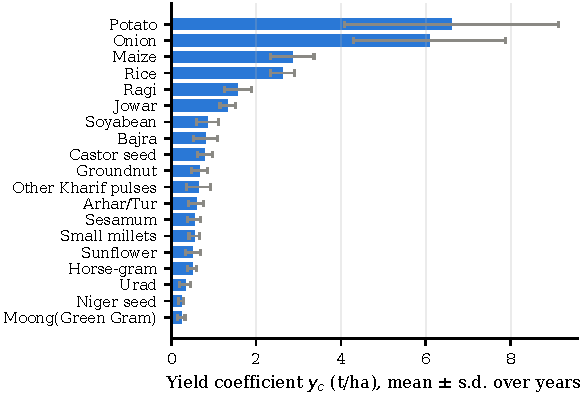
\includegraphics[width=\columnwidth]{fig_coefficients}
\caption{Yield coefficients $y_c$ with year-to-year standard deviation.}
\label{fig:coef}
\end{figure}

\subsection{Optimization 1: Maximum Output}
At $L=\Lhist$, the optimum is $Z^*=11{,}831{,}631$\,t, which is \textbf{21.60\% above} the
historical output (Table~\ref{tab:summary}, Fig.~\ref{fig:opt1}).
\begin{itemize}
  \item \emph{Raised to $m_c$:} Potato, Onion, Maize, Rice, Ragi, Jowar and Soyabean.
  \item \emph{Basic variable:} Bajra, at 330{,}696\,ha. Its yield, 0.808\,t/ha, is the shadow
        price $\lambda^*$: one additional hectare would add about 0.81\,t.
  \item \emph{Held at $a_c$:} all crops with $y_c<\lambda^*$. Their reduced costs
        $y_c-\lambda^*$ (e.g.\ $-0.15$ for Groundnut) give the yield improvement each would need
        before receiving more land.
\end{itemize}

\begin{figure}[t]
\centering
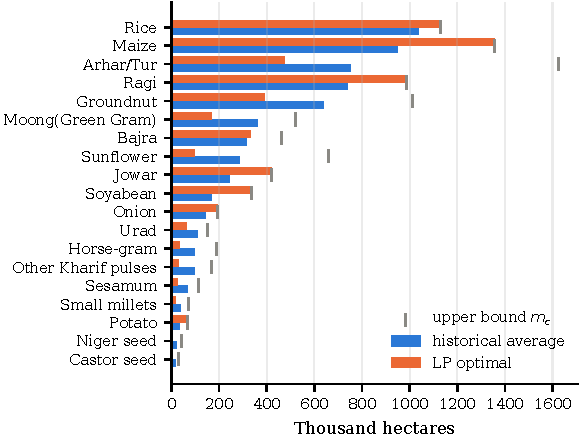
\includegraphics[width=\columnwidth]{fig_opt1_allocation}
\caption{Optimization~1: historical versus LP-optimal hectares per crop at $L=\Lhist$.
Ticks mark the upper bounds $m_c$.}
\label{fig:opt1}
\end{figure}

\subsection{Optimization 2: Minimum Land}
For $D=\Dhist$, the minimum land is 4{,}663{,}668\,ha, a saving of 1{,}461{,}790\,ha
(\textbf{23.86\%}) (Fig.~\ref{fig:opt2}). Rice becomes the basic crop, and
$\mu^*=0.3806$\,ha/t. Solving Opt.~1 at $L=4{,}663{,}668$ returns $Z^*=D$ with
$\lambda^*=2.6273=y_{\text{Rice}}$, so $1/\lambda^*=0.380616=\mu^*$, which verifies
\eqref{eq:dual}. The two models therefore trace the same efficient frontier in opposite
directions.

\begin{figure}[t]
\centering
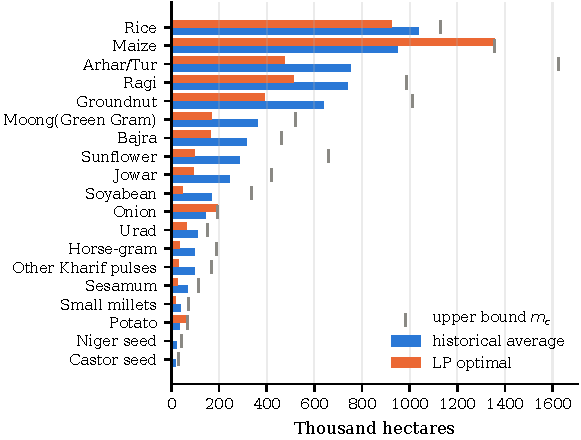
\includegraphics[width=\columnwidth]{fig_opt2_allocation}
\caption{Optimization~2: least-land allocation that meets the historical output $\Dhist$.}
\label{fig:opt2}
\end{figure}

\begin{table}[t]
\centering
\caption{Summary of both models (PuLP--CBC; SciPy--HiGHS identical)}\label{tab:summary}
\begin{tabular}{@{}lrr@{}}
\toprule
 & Historical & LP optimal\\
\midrule
\multicolumn{3}{@{}l}{\emph{Opt.~1, $L=6{,}125{,}458$ ha}}\\
\quad Output (t) & 9{,}729{,}947 & 11{,}831{,}631 \;(+21.60\%)\\
\quad $\lambda^*$ (t/ha), basic crop & -- & 0.808, Bajra\\
\midrule
\multicolumn{3}{@{}l}{\emph{Opt.~2, $D=9{,}729{,}947$ t}}\\
\quad Land (ha) & 6{,}125{,}458 & 4{,}663{,}668 \;($-$23.86\%)\\
\quad $\mu^*$ (ha/t), basic crop & -- & 0.3806, Rice\\
\bottomrule
\end{tabular}
\end{table}

% =====================================================================
\section{Sensitivity Analysis}\label{sec:sens}
% =====================================================================
\subsection{Parametric Land Budget}
$Z^*(L)$ is piecewise linear and concave (Fig.~\ref{fig:param}a). Its slope $\lambda^*(L)$
falls in steps as successive marginal crops reach $m_c$: from about 6.6 (Potato) through
2.9 (Maize), 1.6 (Ragi) and 0.81 (Bajra at $\Lhist$), down to 0 once every crop is at its
upper bound (Fig.~\ref{fig:param}b). This is diminishing marginal returns to land, read
directly from the dual.

\begin{figure*}[t]
\centering
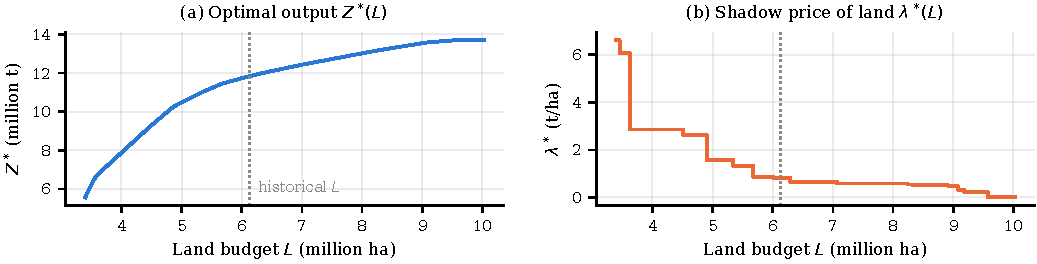
\includegraphics[width=\textwidth]{fig_parametric_land}
\caption{Parametric analysis of Optimization~1. (a) Optimal output versus land budget.
(b) Shadow price of land; each step is a change of the basic (marginal) crop. The dotted
line marks the historical land $\Lhist$.}
\label{fig:param}
\end{figure*}

\subsection{Objective-Coefficient Ranging}
At $\Lhist$, the optimal basis is unchanged as long as:
\begin{itemize}
  \item every crop at $m_c$ keeps $y_c\ge\lambda^*=0.808$;
  \item Bajra (the basic crop) stays within $[0.79,0.86]$;
  \item every crop at $a_c$ keeps $y_c\le0.808$.
\end{itemize}
Soyabean is the most fragile crop at its upper bound: a fall of only 0.05\,t/ha would remove
it from the expanded set.

\subsection{Yield-Shock Scenarios}
Table~\ref{tab:shock} shows that a uniform shock only rescales $Z^*$, so the plan is robust
to a generally good or bad year. A crop-specific shock re-allocates land only for crops near
the margin, as the ranging analysis predicts.

\begin{table}[t]
\centering
\caption{Yield-shock scenarios (Opt.~1 at $\Lhist$)}\label{tab:shock}
\begin{tabular}{@{}lrrr@{}}
\toprule
Scenario & Shock & $\Delta Z^*$ & ha re-allocated\\
\midrule
All crops & $-30\%$ & $-30.00\%$ & 0\\
All crops & $+15\%$ & $+15.00\%$ & 0\\
Maize only & $-30\%$ & $-9.81\%$ & 0\\
Rice only & $-30\%$ & $-7.53\%$ & 0\\
Soyabean only & $-30\%$ & $-0.40\%$ & 288{,}406\\
Soyabean only & $-15\%$ & $-0.27\%$ & 158{,}069\\
\bottomrule
\end{tabular}
\end{table}

\subsection{Flexibility Required for the Gain}
Historical min--max bounds are wide: some crop areas varied three- to four-fold over 22
years. Replacing \eqref{eq:bounds} with $(1-p)\bar{x}_c\le x_c\le(1+p)\bar{x}_c$ shows
that the gain grows almost linearly in $p$ (Fig.~\ref{fig:band}). With $p=10\%$, the gain
is 6.2\% more output or 5.0\% less land, consistent with the 3.75--15\% reported
in~\cite{supriya2022}.

\begin{figure}[t]
\centering
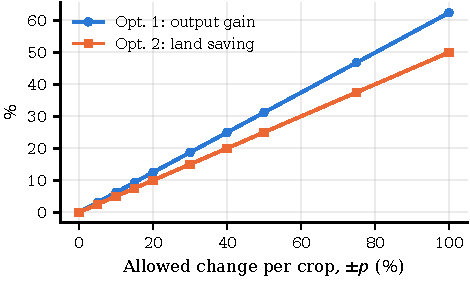
\includegraphics[width=\columnwidth]{fig_band_sweep}
\caption{Gain when every crop may move at most $\pm p\%$ from its historical area.}
\label{fig:band}
\end{figure}

% =====================================================================
\section{Multi-District Comparison}\label{sec:multi}
% =====================================================================
Both LPs were solved independently for each of 27 Karnataka districts, each with its own
coefficients, bounds, $\Lhist$ and $\Dhist$ (Fig.~\ref{fig:multi}). The median output gain
is 25.8\% and the median land saving is 24.4\%.
\begin{itemize}
  \item \emph{Largest potential:} the diverse, dry northern districts, i.e.\ Koppal (+65\%),
        Gadag (+55\%) and Raichur (+48\%).
  \item \emph{Smallest potential:} the coastal rice districts Udupi (+0.2\%) and Dakshina
        Kannada (+0.6\%), which grow essentially two crops.
\end{itemize}
Maize is the crop the LP expands most often (16 of 27 districts), and the gain is positively
correlated with the number of crops grown ($r=0.50$).

\begin{figure}[t]
\centering
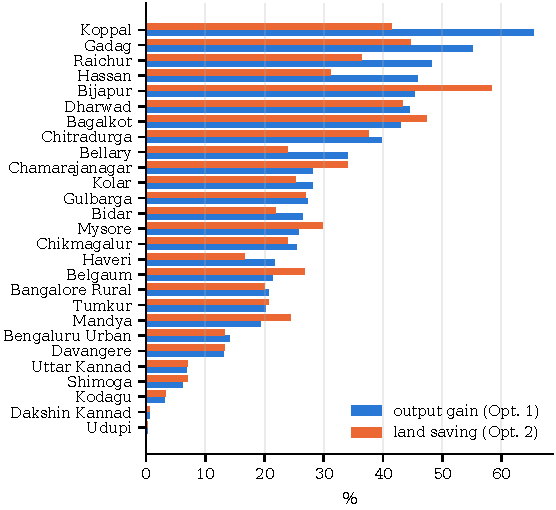
\includegraphics[width=\columnwidth]{fig_multi_district}
\caption{LP improvement by district (Karnataka, Kharif, 1998--2019).}
\label{fig:multi}
\end{figure}

% =====================================================================
\section{Decision-Support Dashboard}\label{sec:tool}
% =====================================================================
The models are delivered as \emph{CropLP}, a web application (Fig.~\ref{fig:arch}). A FastAPI
backend exposes the same \texttt{or\_core} module as a JSON API, so the browser shows exactly
the numbers reported here. The frontend is a guided, eight-step interface that runs fully
offline. A user can drag and drop any CSV or Excel file whose minimum columns are crop, area
and production; column names are mapped automatically and can be edited. The pipeline of
Fig.~\ref{fig:workflow} then runs live across the following steps:
\begin{itemize}
  \item data quality, with a plain-language cleaning log;
  \item exploratory insights (auto-generated insight cards, yield trends, district heat-maps,
        best crop per district and season);
  \item crop selection with per-crop unit badges and the LP coefficients;
  \item the two LPs, driven by sliders, with a plain-English explanation of each plan, the
        printed model, a solver cross-check and CSV export;
  \item a what-if page (parametric curves, ranging, a weather-shock simulator);
  \item the multi-district comparison;
  \item the method and a glossary.
\end{itemize}
Every cleaning rule, scope, averaging method and bound type can be changed interactively.

\begin{figure}[t]
\centering
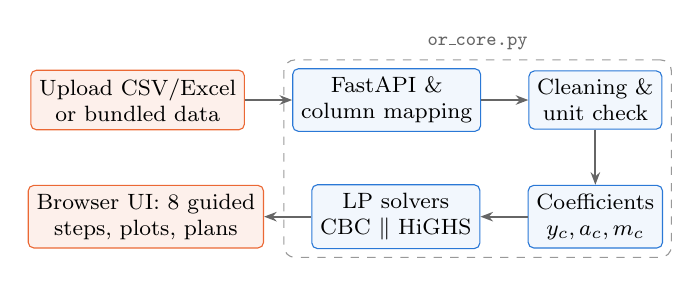
\begin{tikzpicture}[font=\footnotesize,
  blk/.style={draw=orblue, fill=orblue!6, rounded corners=2pt, align=center, minimum height=6mm, inner sep=3pt},
  io/.style={draw=ororange, fill=ororange!10, rounded corners=2pt, align=center, minimum height=6mm, inner sep=3pt},
  arr/.style={-{Stealth[length=1.6mm]}, thick, draw=black!60}]
\node[io] (up) {Upload CSV/Excel\\or bundled data};
\node[blk, right=6mm of up] (map) {FastAPI \&\\column mapping};
\node[blk, right=6mm of map] (cl) {Cleaning \&\\unit check};
\node[blk, below=7mm of cl] (co) {Coefficients\\$y_c,a_c,m_c$};
\node[blk, left=6mm of co] (lp) {LP solvers\\CBC $\Vert$ HiGHS};
\node[io, left=6mm of lp] (ui) {Browser UI: 8 guided\\steps, plots, plans};
\draw[arr] (up) -- (map); \draw[arr] (map) -- (cl); \draw[arr] (cl) -- (co);
\draw[arr] (co) -- (lp); \draw[arr] (lp) -- (ui);
\node[draw=black!40, dashed, rounded corners, fit=(map)(cl)(co)(lp), inner sep=3pt,
      label={[font=\scriptsize, text=black!60]above:\texttt{or\_core.py}}] {};
\end{tikzpicture}
\caption{Architecture of the CropLP web application. All computation lives in a single
reusable module shared by the dashboard and the batch case-study script.}
\label{fig:arch}
\end{figure}

% =====================================================================
\section{Validation on Synthetic Data}\label{sec:valid}
% =====================================================================
A seeded generator produces a fictitious state with 6 districts, 3 seasons, 21 crops and
the years 2008--2019. It includes district-specific comparative advantage, a yield trend,
weather noise and a Kharif drought in 2015, and it deliberately plants every quirk the
pipeline must catch. All of them are detected (Table~\ref{tab:synth}).

On the synthetic Kharif scope, Opt.~1 gains 5.15\% and Opt.~2 saves 4.74\%, and the two
solvers agree exactly. A second file with only four, differently named columns (crop, year,
area, production) is mapped automatically and reproduces the corresponding district result
(+12.07\%) of the full file.

\begin{table}[t]
\centering
\caption{Planted quirks in the synthetic dataset}\label{tab:synth}
\begin{tabular}{@{}lll@{}}
\toprule
Planted quirk & Caught by & Outcome\\
\midrule
8 duplicate rows & cleaning & removed\\
25 zero-production rows & cleaning & removed\\
144 ``Total foodgrain'' rows & cleaning & removed\\
``Paddy'' alias of Rice & alias merge & merged\\
Coconut (nuts), Cotton (bales) & unit check & excluded\\
2015 Kharif drought & quirk detector & flagged\\
\bottomrule
\end{tabular}
\end{table}

% =====================================================================
\section{Discussion and Limitations}\label{sec:disc}
% =====================================================================
\begin{enumerate}
  \item \textbf{Weight-based objective.} A tonne of onion counts the same as a tonne of pulses,
        so heavy, high-moisture crops are favoured and protein-dense pulses are cut to their
        minimum. The objective measures output, not profit or nutrition, because the dataset has
        no price or cost field.
  \item \textbf{Bounds drive the answer.} In a knapsack-structured LP, $a_c$ and $m_c$ decide
        how far the plan moves. Historical bounds give an optimistic +21.6\%; a $\pm10\%$ band gives
        +6.2\%. Both figures are reported.
  \item \textbf{Historical averages.} Weather is not modelled in the base LP. The shock analysis
        shows the plan is robust to uniform shocks but sensitive at the margin.
  \item \textbf{Not modelled:} soil, irrigation, labour, crop rotation, prices and demand, and
        food-security requirements.
  \item \textbf{Data quality.} Without the reconciliation of Sec.~\ref{sec:stacked}, every
        coefficient would mix two scales. Any study that uses this public file should apply it.
\end{enumerate}

% =====================================================================
\section{Conclusion and Future Work}\label{sec:concl}
% =====================================================================
Using only area, production and yield from a public government record, two dual LP
models of crop-area allocation were built, solved, cross-validated and analysed. For
Karnataka's Kharif season, historical land could have produced 21.6\% more output, or
historical output could have been grown on 23.9\% less land. A realistic $\pm10\%$
re-planning still yields about 6\%. The gains are concentrated in diverse dryland
districts.

A previously unreported stacked-duplicate defect in the public dataset was identified and
repaired automatically. The complete pipeline is available as an upload-driven dashboard.

Future work will:
\begin{itemize}
  \item add price- or nutrition-weighted objectives;
  \item add rotation and minimum-pulse constraints;
  \item develop a stochastic or robust LP using the computed yield variances;
  \item build a state-wide model linking district LPs through shared food-security constraints.
\end{itemize}

% =====================================================================
\begin{thebibliography}{00}
\bibitem{taha2017} H.~A.~Taha, \emph{Operations Research: An Introduction}, 10th~ed. Pearson, 2017.
\bibitem{wankhade2012} S.~Wankhade and H.~Lunge, ``LP technique for optimum resource allocation in agricultural production, Akola district, Maharashtra,'' 2012.
\bibitem{majeke2020} F.~Majeke \textit{et~al.}, ``Linear programming approach---application in agriculture,'' 2020.
\bibitem{supriya2022} S.~Supriya \textit{et~al.}, ``Optimal crop plans using LP in Jayashankar Bhupalpally district, Telangana,'' 2022.
\bibitem{paidipati2017} K.~K.~Paidipati and S.~R.~Padi, ``Optimal programming problems for crop planning and agricultural resource management,'' 2017.
\bibitem{liang2023} X.~Liang, ``LP approach in agricultural production-land allocation,'' Springer, 2023.
\bibitem{moafw} Ministry of Agriculture \& Farmers Welfare, Government of India, \emph{District-wise, Season-wise Crop Production Statistics (1997--2020-21)}, data.gov.in, via Kaggle.
\bibitem{dantzig1957} G.~B.~Dantzig, ``Discrete-variable extremum problems,'' \emph{Operations Research}, vol.~5, no.~2, pp.~266--288, 1957.
\bibitem{pulp} S.~Mitchell, M.~O'Sullivan, and I.~Dunning, ``PuLP: A linear programming toolkit for Python,'' The University of Auckland, 2011.
\bibitem{cbc} J.~Forrest and R.~Lougee-Heimer, ``CBC user guide,'' in \emph{Emerging Theory, Methods, and Applications}, INFORMS, 2005, pp.~257--277.
\bibitem{scipy} P.~Virtanen \textit{et~al.}, ``SciPy 1.0: Fundamental algorithms for scientific computing in Python,'' \emph{Nature Methods}, vol.~17, pp.~261--272, 2020.
\bibitem{highs} Q.~Huangfu and J.~A.~J.~Hall, ``Parallelizing the dual revised simplex method,'' \emph{Mathematical Programming Computation}, vol.~10, no.~1, pp.~119--142, 2018.
\end{thebibliography}

\end{document}
